\begin{figure}[H]
\centering
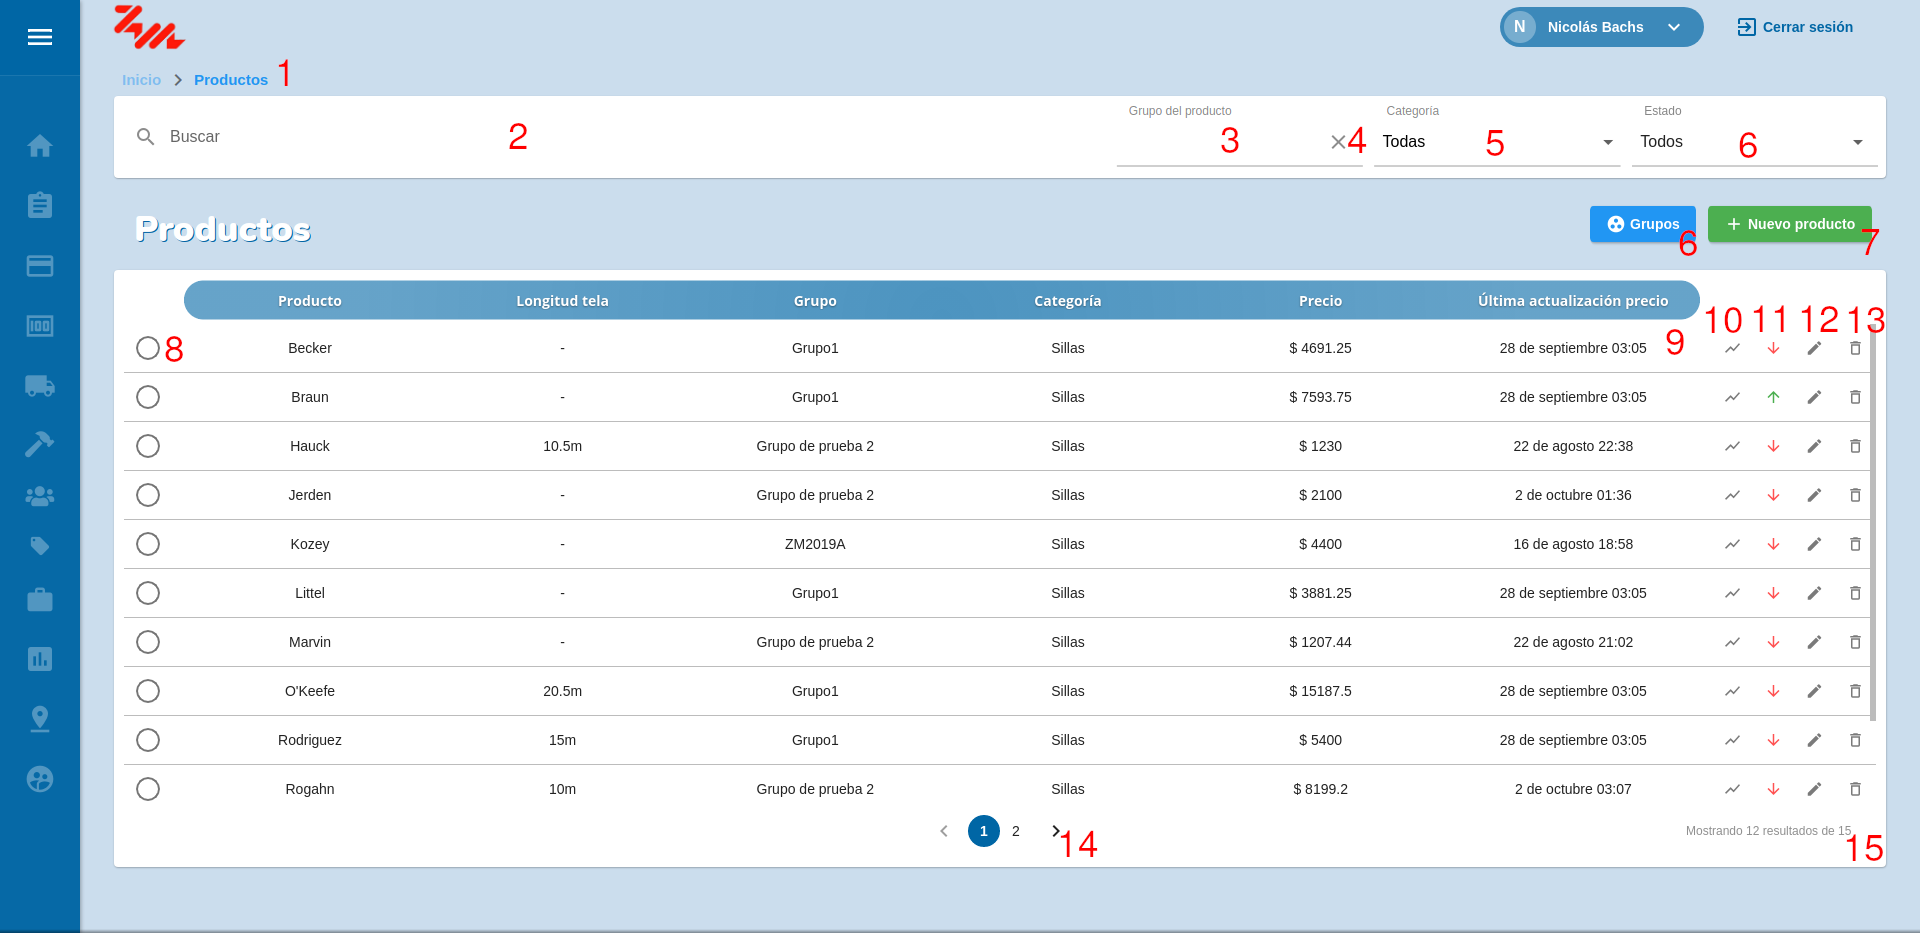
\includegraphics[width=\textwidth,height=\textheight,keepaspectratio]{Escenarios/AD-42-00}
\caption{Escenario - AD-42-00}
\label{fig:AD-42-00}
\end{figure}

Este escenario muestra toda la información referida a los productos, junto con las acciones disponibles.
El botón \textbf{AD-42-01} permite navegar al escenario \textbf{AD-02-00}. El campo \textbf{AD-42-02} permite ingresar un texto para filtrar los productos por nombre, el campo \textbf{AD-42-03} permite ingresar un grupo de producto para filtrar los productos que pertenezcan a dicho grupo, el campo el campo cuenta con el botón \textbf{AD-42-04} que permite borrar el texto ingresado en el campo, la lista desplegable \textbf{AD-42-05} permite al usuario filtrar por la categoría a la cual pertenece el producto y la lista desplegable \textbf{AD-42-05} permite al usuario filtrar por los estados en los cuales puede encontrarse el producto.

El botón \textbf{AD-42-06} permite al usuario gestionar los grupos de productos, navegando al escenario \textbf{AD-45-00}. El botón \textbf{AD-42-07} permite al usuario crear un nuevo producto y navega al escenario \textbf{AD-43-00}.
El botón \textbf{AD-42-08} permite al usuario seleccionar uno o más productos del resultado de la búsqueda. Si existen productos seleccionados se mostrarán botones con las opción de borrar o activar/desactivar según corresponda. El campo \textbf{AD-42-09} muestra la información relacionada a los productos especificando el código, nombre del producto, longitud de tela, grupo al que pertenece, precio actual y cuándo se realizó la última actualización del precio. El botón \textbf{AD-42-10} permite navegar al escenario \textbf{AD-44-00} para ver los precios del producto, el botón \textbf{AD-42-11} permite al usuario dar de alta/baja un producto, el botón \textbf{AD-42-12} permite al usuario editar el producto navegando al escenario \textbf{AD-43-00} y el botón \textbf{AD-42-18} permite al usuario borrar el producto. 
En \textbf{AD-42-14} se mostrarán las páginas de resultado, pudiendo cambiar de página. En \textbf{AD-42-15} se mostrará cuantos resultados se están visualizando y el total.
\clearpage
